\usetikzlibrary{arrows.meta,calc}
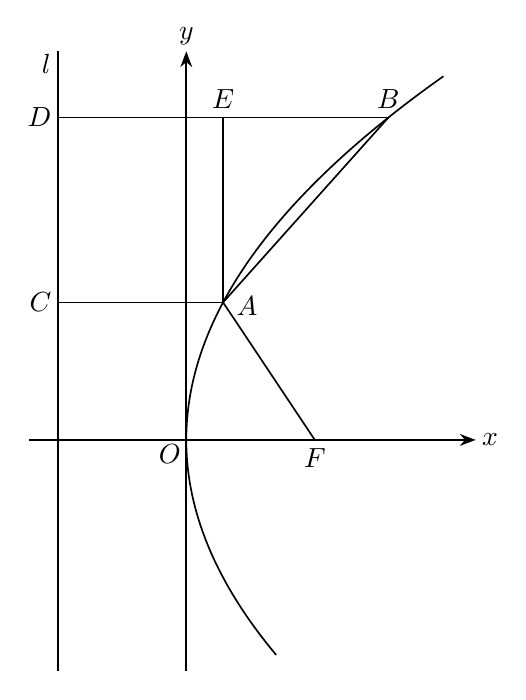
\begin{tikzpicture}[x=1.05cm,y=1.05cm,line width=.6pt,font=\normalsize,>=Stealth]
\def\parp{3.1100423}
\coordinate (O) at (0,0);
\coordinate (F) at (1.5550212,0);
\coordinate (A) at (0.4449788,1.6636724);
\coordinate (B) at (2.4449788,3.8997404);
\coordinate (C) at (-1.5550212,1.6636724);
\coordinate (D) at (-1.5550212,3.8997404);
\coordinate (E) at (0.4449788,3.8997404);
\draw[->] (-1.9,0)--(3.5,0) node[right,inner sep=0pt,xshift=2pt] {$x$};
\draw[->] (0,-2.8)--(0,4.7) node[above,inner sep=0pt,yshift=2pt] {$y$};
\draw (-1.5550212,-2.8)--(-1.5550212,4.7);
\draw plot[domain=-2.6:4.4,samples=121,variable=\t] ({\t*\t/(2*\parp)},\t);
\draw (A)--(B);
\draw (A)--(C);
\draw (B)--(D);
\draw (A)--(E);
\draw (A)--(F);
\node[anchor=west,inner sep=0pt] at (0.60,1.62) {$A$};
\node[anchor=south,inner sep=0pt,yshift=3pt] at (B) {$B$};
\node[anchor=east,inner sep=0pt,xshift=-2pt] at (C) {$C$};
\node[anchor=east,inner sep=0pt,xshift=-2pt] at (D) {$D$};
\node[anchor=south,inner sep=0pt,yshift=3pt] at (E) {$E$};
\node[anchor=north,inner sep=0pt,yshift=-3pt] at (F) {$F$};
\node[anchor=east,inner sep=0pt] at (-1.63,4.55) {$l$};
\node[anchor=center,inner sep=0pt] at (-0.20,-0.17) {$O$};
\end{tikzpicture}
